\chapter{Reconfigurations}

By the beginning of 1978, Ajahn Sumedho had departed Thailand and was
engaged in establishing a branch monastery in Britain. The tall American
ex-helicopter pilot who was skilled in crochet, Ajahn Pabakharo, had
been asked by Tan Ajahn Chah to take over leading the community at Wat
Pah Nanachat.

Around the beginning of 1978 a young, energetic, smiley English fellow
called Jeremy had arrived and was expressing interest in joining the
community. One morning, when he was diligently using a machete to chop
wood at the kitchen, he accidentally missed the piece of wood and
instead hacked into his foot. The reason I remember the incident is
because it fell to me to accompany him to see a doctor. In fact I ended
up physically carrying him into the local hospital. Jeremy was one of
those visitors who did settle in and make a commitment. He eventually
received \emph{upasampada} from Tan Ajahn Chah and the sangha at Wat Pah
Pong and was given the name Amaro Bhikkhu.

My carrying the not insignificant weight of Jeremy into hospital may or
may not have contributed to later that year myself entering hospital for
knee surgery. More likely it was down to the motorbike accident,
combined with hours of forcing myself to sit on the floor without a
cushion. I had gone to Bangkok to see if there was anything that could
be done about the increasing amount of pain I was having with my knees,
and the advice I received was that I needed a meniscectomy. In those
days that amounted to open surgery on both legs, and resulted in my
being in Ramathibodi hospital with both legs in full length plaster
casts for several weeks. Once the casts had been removed it became
apparent that the excessive growth of scar tissue had caused both knee
joints to seize up, requiring two more sessions of general anaesthetic
so the scar tissue could be torn. That was an ordeal I would not want to
have to repeat. Initially I had been told by the doctor that having both
knees done at the same time might mean being incapacitated for something
like three or four weeks. As it happened it was many weeks.

To my surprise, one day as I lay in bed in the hospital, I received a
visitor; it was ex-Tan Jotiko, now calling himself Mason Hamilton. When
Ajahn Sumedho had left for Britain the then Tan Jotiko had gone to live
at another, rather remote branch monastery called Wat Keurn. It wasn't
long, however, before he took the decision to renounce his commitment to
the robes and return to lay life. Of course, I was sad to see my friend
in this new form, but as far as I recall that it wasn't too big a deal.
Tan Varapañño had already disrobed by that time, so the perception
wasn't new, and finding myself stuck all alone in a Bangkok hospital for
weeks on end meant that I was already dealing with plenty of
disappointment; this was just a bit more.

Mason was staying with Geoff, an English friend and supporter of Wat Pah
Nanachat, and by the time I emerged from hospital the two of them had
organized a trip up to the north of Thailand, to Chiangmai. There we
would have the use of a quiet secluded house on the side of a forested
hill.

Before departing on that trip I had a chance to pay my respects to Tan
Ajahn Chah, who himself was in hospital in Bangkok. Seeing him again
meant a great deal. Having been for such a long time away from the
mother ship and its captain, it was encouraging to see Tan Ajahn Chah
once more. My knees were still not very flexible, so when I attempted to
get down on the floor to bow, I could hardly have been more awkward. I
started telling Tan Ajahn Chah, `It shouldn't be this way. The doctors
said it would only take a few weeks and here I am after all this time
and my knees are still not working properly.' He looked at me sternly,
and with an almost surprised expression at the degree of my foolishness
said, `What do you mean it shouldn't be this way? If it shouldn't be
this way it wouldn't be this way!' That was helpful. Thank you, Tan
Ajahn Chah. He wasn't implying anything like there being a big plan and
that the universe was teaching me a lesson; he was simply saying there
are causes and conditions for it to be this way, so stop resisting
reality. It \emph{is} like this! Such resistance only makes things
worse.

Mason, Geoff and I had a splendid road trip. The house on the side of
the hill, Doi Suthep, was Japanese-style and was surrounded by gorgeous
gardens and forest. Nearby was a waterfall that we could easily walk to.
During the day Geoff would sometimes drive us around to see some of the
sights, and at night it was quiet -- no more of the noise and fumes of
Bangkok traffic. That interlude was refreshing and renewing; thank you,
Geoff.

On one of those trips out, Geoff, Mason and I went as far as the next
province, Chiang Rai, where there was a small hermitage monastery
associated with Wat Pah Pong, called Wat Doi Dhamma Chedi. The abbot
there was Ajahn Koon, a short, young, enthusiastic and incredibly
talkative monk. Besides the welcome we received, there was a nearby
thermal hot pool where I was able to soak my still painful limbs. Ajahn
Koon generously invited me to stay there for the approaching Rains
Retreat (\emph{pansah}) and the thought of having access to the thermal
spring clinched it for me.

It was appropriate that I return to Wat Pah Nanachat to get permission
to be away for the Rains. By the time I reached there, there had been
another change in leadership. Now Ajahn Jagaro had been put in charge.
He was an Australian whose family were of Italian descent and he had a
big warm heart. He didn't hesitate to draw lines when they were needed,
but he did so with a warmth and sensitivity that commanded love and
respect from the community. There seemed to be no hesitation in giving
me permission to return to Chiang Rai province in the North.

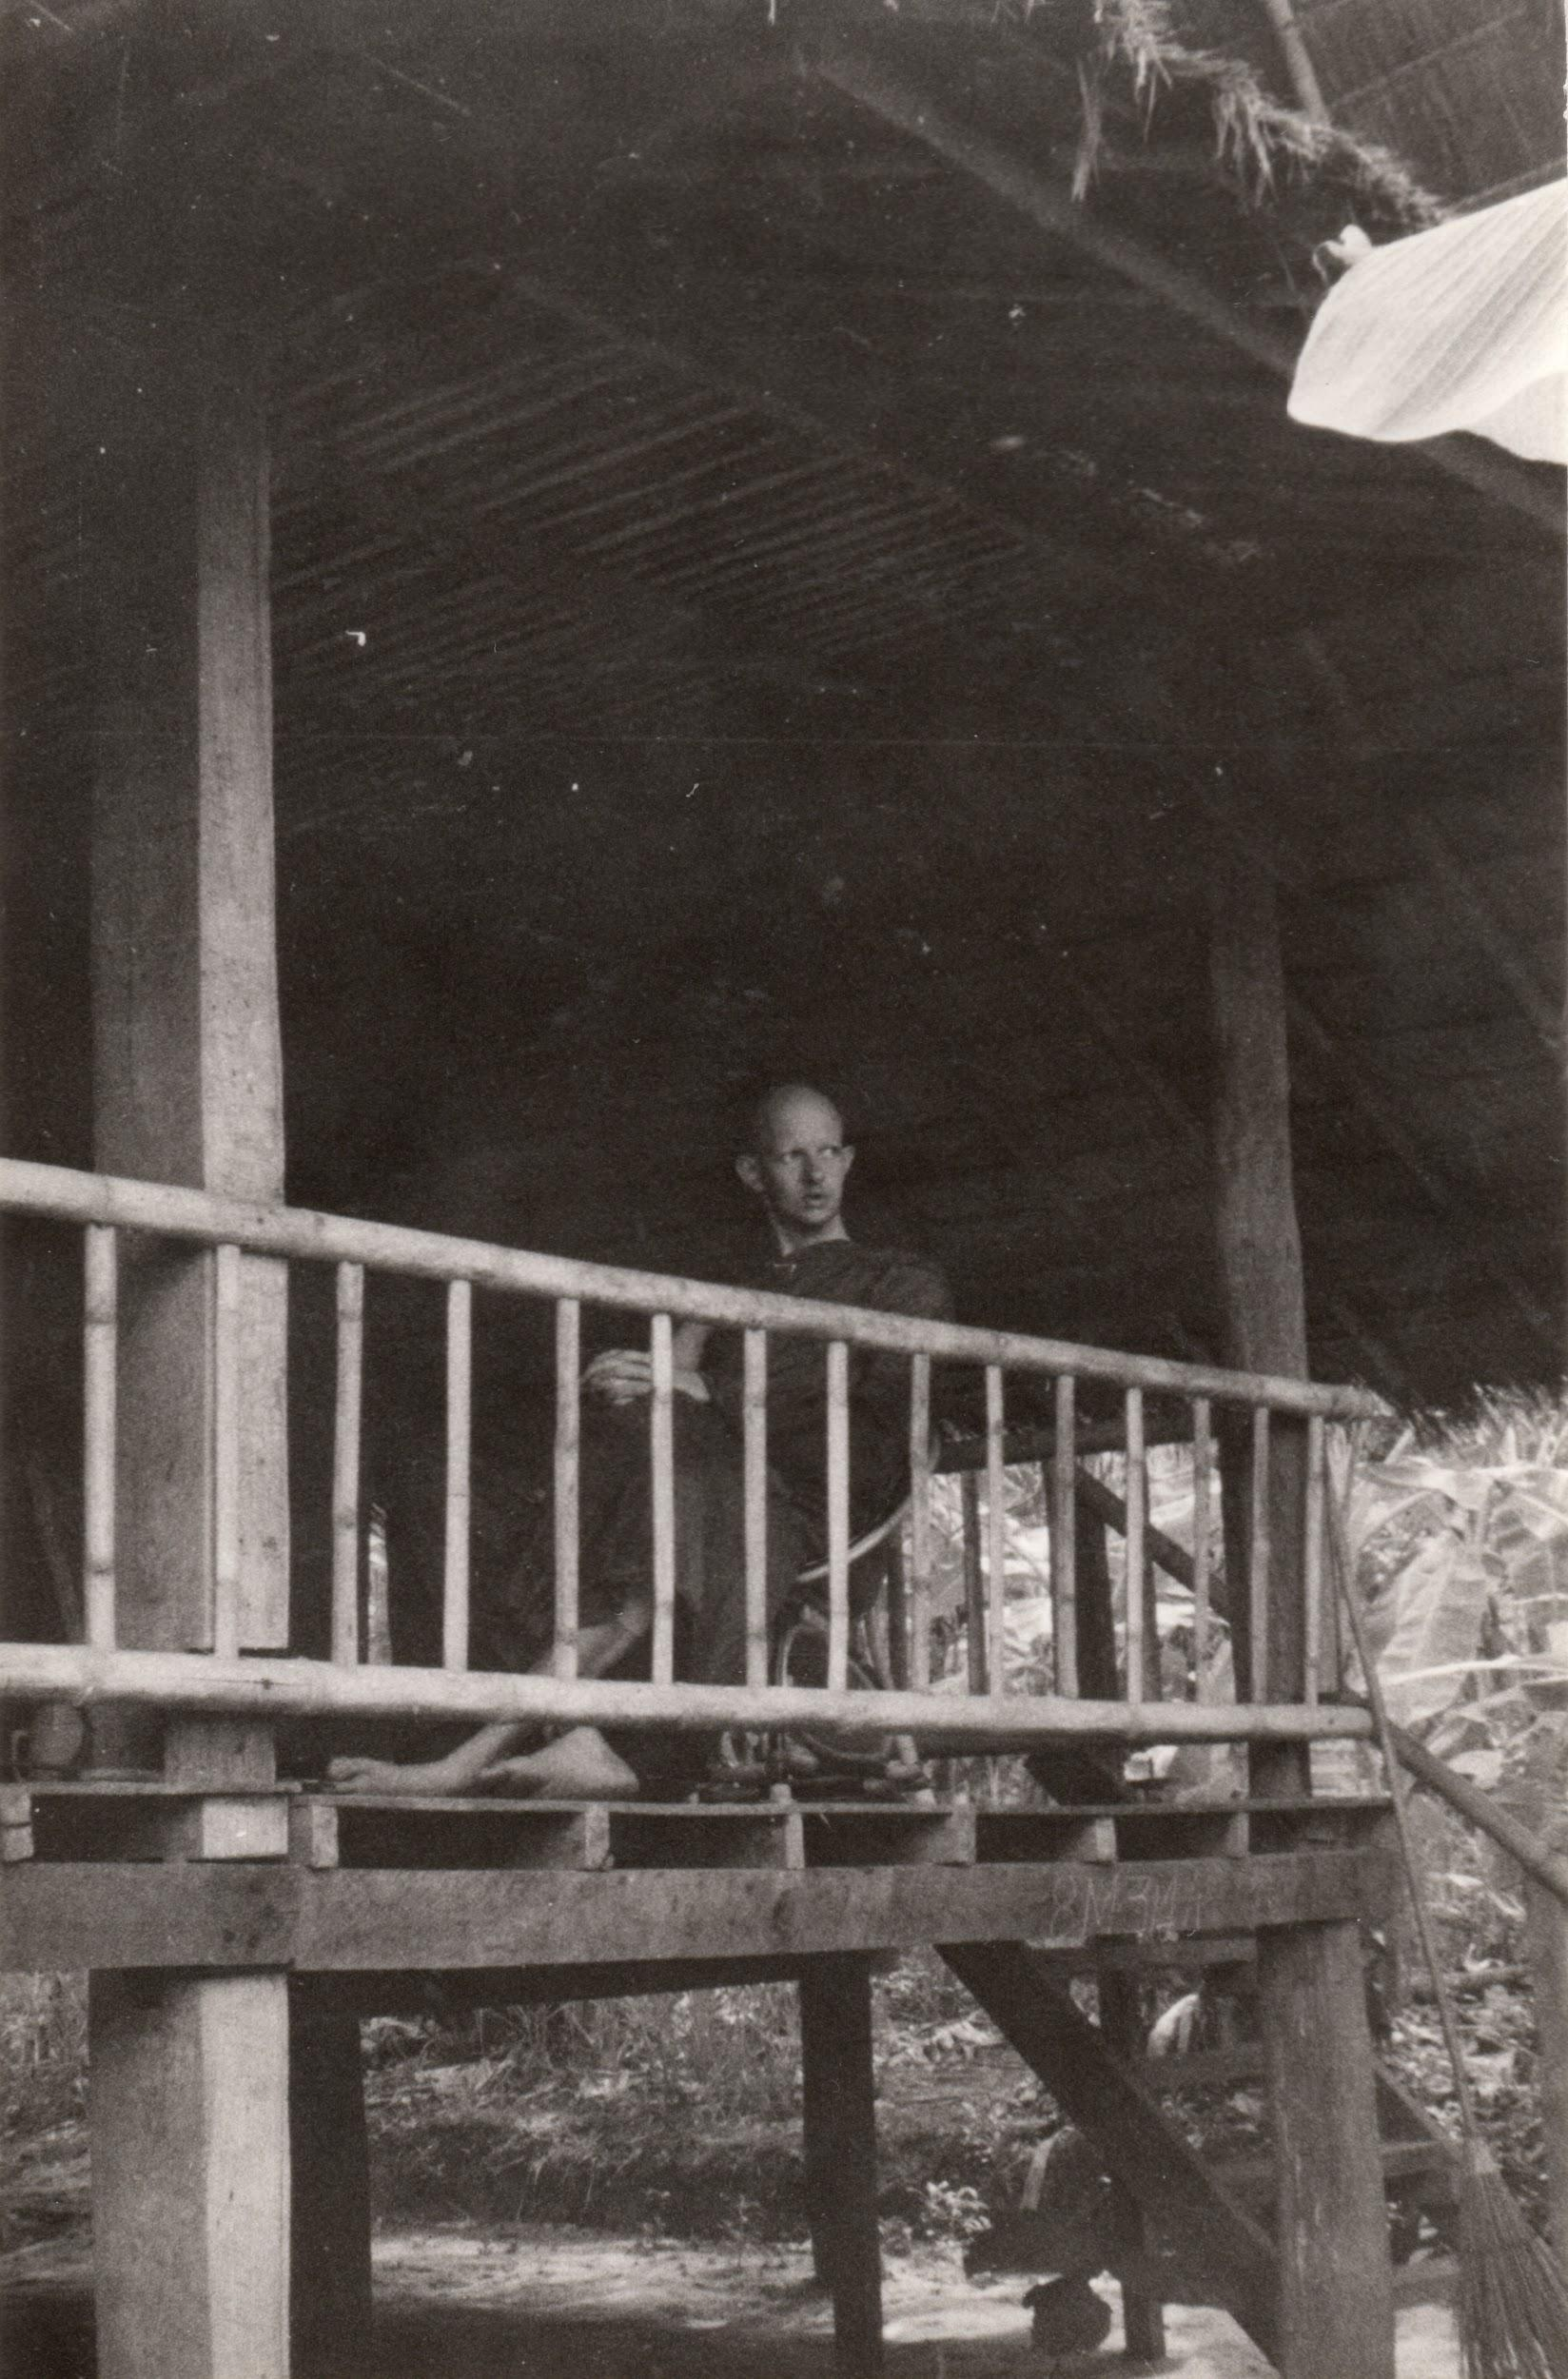
\includegraphics[width=\linewidth]{image3.jpeg}

